\documentclass[11pt]{report}

\usepackage{amsmath,amsfonts,amssymb}
\usepackage{graphicx}
\usepackage[colorlinks=true, allcolors=blue]{hyperref}
\usepackage{listings}
\usepackage{tcolorbox}
\usepackage[top=1in,bottom=1in,left=0.5in,right=0.5in]{geometry}
\usepackage{graphicx}
\usepackage{authblk}
\usepackage{amsmath, amsfonts, graphicx, placeins}
\usepackage{amssymb}% for \sphericalangle
\usepackage{braket}
\usepackage{subcaption}
\usepackage{mathtools}
\usepackage{breqn}
\usepackage{hyperref}
\usepackage{rotating}
\usepackage{multirow}
\usepackage{color}
\usepackage{placeins}
\usepackage{todonotes}


\lstset{ 
basicstyle=\linespread{0.8}\scriptsize,
commentstyle=\color{gray},
frame=single,
numbers=left,
tabsize=2
}


\begin{document} 

{\LARGE\centering
Review notes for “Characterization of Multianode Photomultiplier Tubes for use in the CLAS12 RICH Detector”\\[1cm]

June 2022\\[1cm]
}

\begin{tcolorbox}[enlarge top by=2em,colbacktitle=black!60!white,colframe=black!80!white,left=0pt,right=0pt,top=0pt,bottom=0pt,boxrule=0.3pt,title=\bfseries1.01]
Line 39: “With a high quantum efficiency in the visible light region” – it might be good to provide a number (for example, 30\% at 450 nm, or something like that) here because ‘high’ can be relative.
\end{tcolorbox}

\fbox{The text of the paper was changed to address the comment. See before and after version below:}

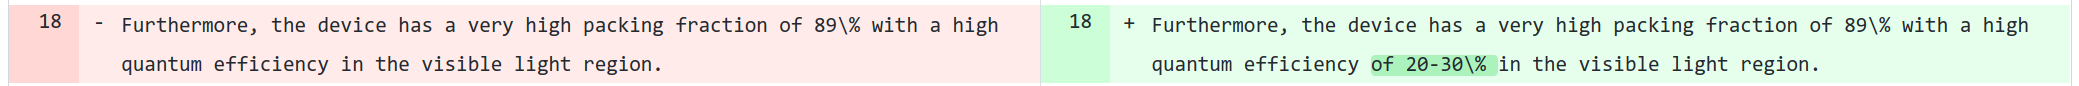
\includegraphics[width=\linewidth]{round1/1.01.png}

\begin{tcolorbox}[enlarge top by=2em,colbacktitle=red!60!white,colframe=black!80!white,left=0pt,right=0pt,top=0pt,bottom=0pt,boxrule=0.3pt,title=\bfseries1.02]
Fig  10+11:  It  is  difficult  to  clearly  observe  the  various  features  in  the  plots.   Additionally,  there  is no indication in the Figure caption which side of the dashed red line is being cut.  The central figure should have units on the y-axis (counts or arb.  units).  The central figure should probably have the same x-axis range as the other figures in the panel.  Similarly for Fig 11.
\end{tcolorbox}

The resolutions of Fig 10+11 were improved, a label was added to the central figures of both, and the axes ranges were made consistent throughout. Additionally, more text was added to the captions for both figures to address which side of the dashed red line is cut and to clarify the signature of the crosstalk in the neighboring pixels.

\begin{tcolorbox}[enlarge top by=2em,colbacktitle=black!60!white,colframe=black!80!white,left=0pt,right=0pt,top=0pt,bottom=0pt,boxrule=0.3pt,title=\bfseries1.03]
Line 234:  Where does this tabulated efficiency of the photodiode come from?  Are there uncertainties on this number?
\end{tcolorbox}

The number comes from the Hamamatsu specifications datasheet. No uncertainties may be found there, and in such case the understanding is that all the digits in the number are meaningful. The text of the paper was changed to address the comment. See before and after version below.

\fbox{\bfseries The text of the paper was changed to address the comment. See before and after version below:}
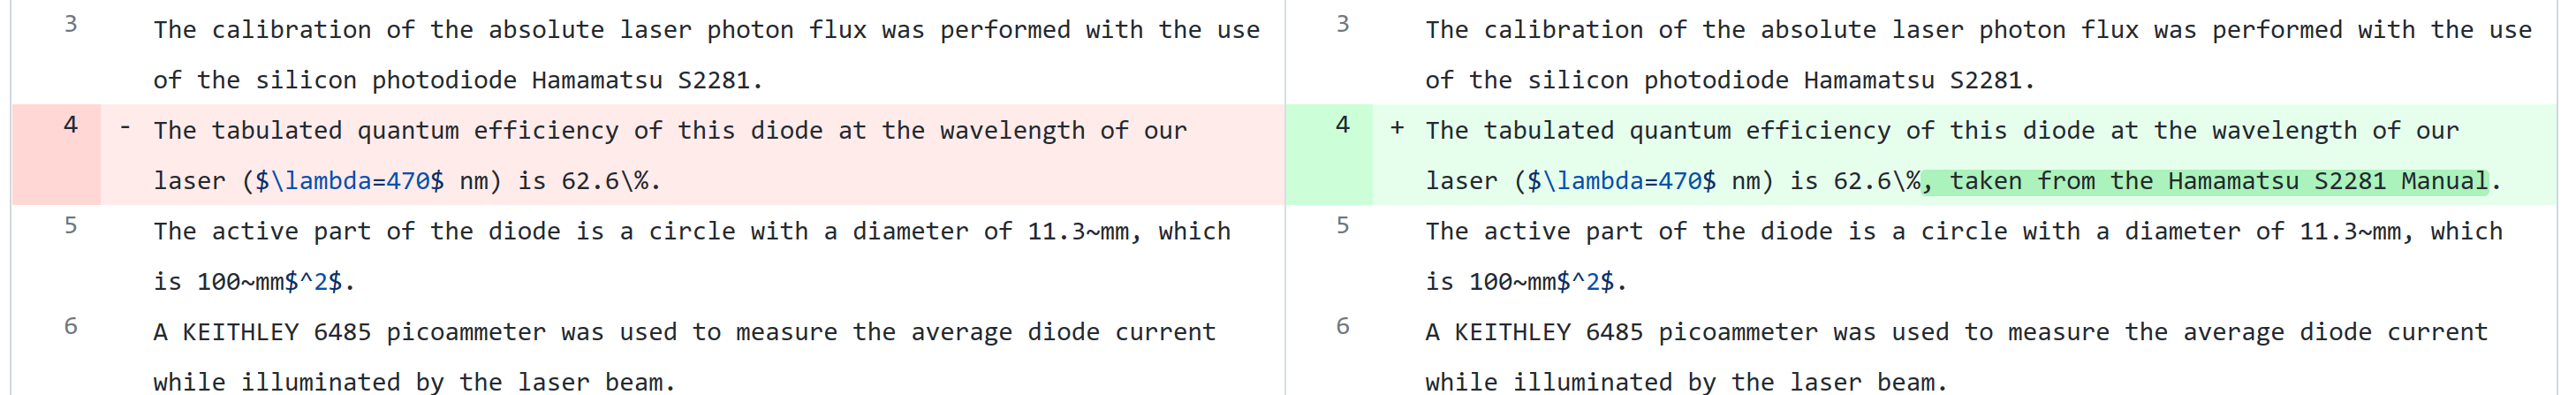
\includegraphics[width=\linewidth]{round1/1.03.png}

\begin{tcolorbox}[enlarge top by=2em,colbacktitle=black!60!white,colframe=black!80!white,left=0pt,right=0pt,top=0pt,bottom=0pt,boxrule=0.3pt,title=\bfseries1.04]
Fig  12  caption:  Needs  a  bit  of  rewriting,  its  currently  poorly  worded.   For  example:The light intensity distribution dN/dS, defined as ..., for a row of three MaPMTs in the laser stand.
\end{tcolorbox}

\fbox{\bfseries The text of the paper was changed to address the comment. See before and after version below:}

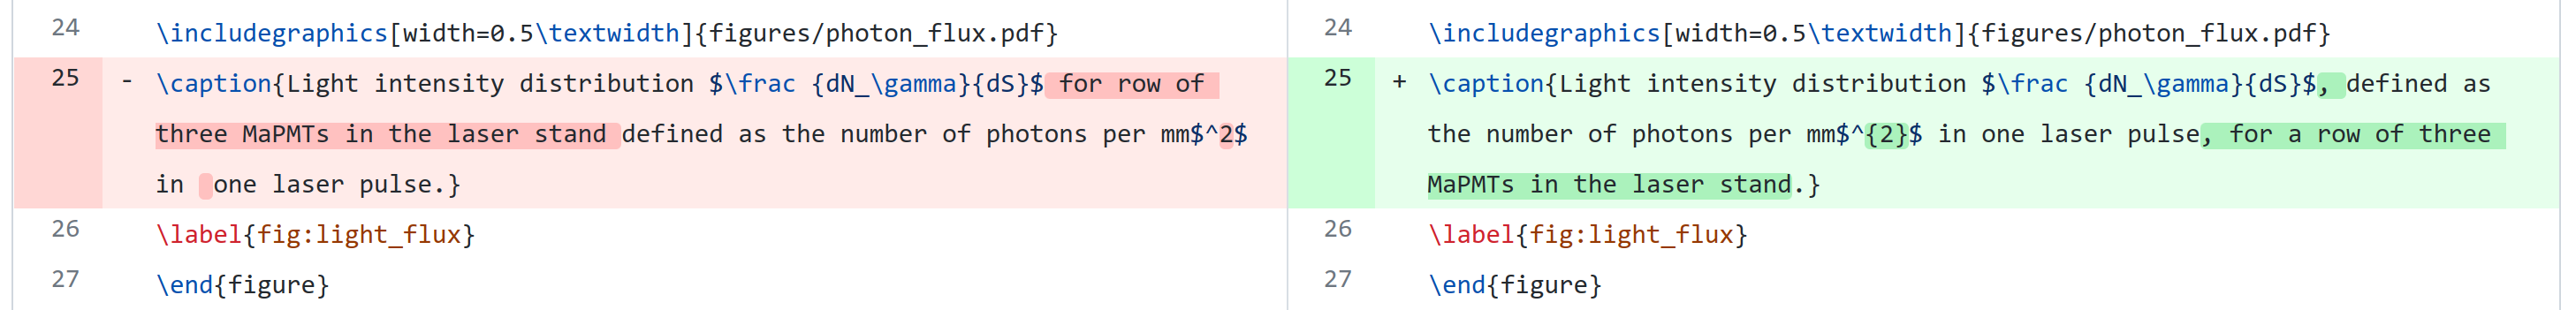
\includegraphics[width=\linewidth]{round1/1.04.png}

\begin{tcolorbox}[enlarge top by=2em,colbacktitle=black!60!white,colframe=black!80!white,left=0pt,right=0pt,top=0pt,bottom=0pt,boxrule=0.3pt,title=\bfseries1.05]
Line 253:  Issue with math mode?  Why are the units italicized?
\end{tcolorbox}

\fbox{\bfseries The text of the paper was changed to address the comment}

\begin{tcolorbox}[enlarge top by=2em,colbacktitle=black!60!white,colframe=black!80!white,left=0pt,right=0pt,top=0pt,bottom=0pt,boxrule=0.3pt,title=\bfseries1.06]
Line 263:  Are there other efficiencies to consider?  For example, what is the collection efficiency (the  efficiency  for  successfully  converting  the  generated  PE  at  the  photocathode  to  a  signal  at  the anode – which might be non-unity due to inefficiencies collecting the first PE at the first dynode).
\end{tcolorbox}

\fbox{\bfseries The text of the paper was changed to address the comment. See before and after version below:}

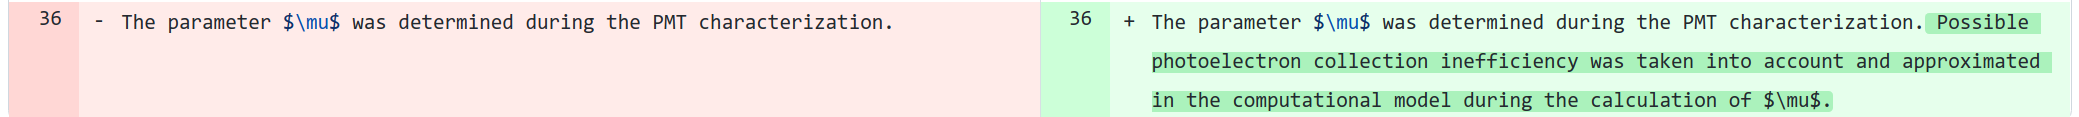
\includegraphics[width=\linewidth]{round1/1.06.png}

\begin{tcolorbox}[enlarge top by=2em,colbacktitle=black!60!white,colframe=black!80!white,left=0pt,right=0pt,top=0pt,bottom=0pt,boxrule=0.3pt,title=\bfseries1.07]
Line 287:  I do not think the parameters, such as scale and gain, need to be italicized.
\end{tcolorbox}

\fbox{\bfseries The text of the paper was changed to address the comment.}

\begin{tcolorbox}[enlarge top by=2em,colbacktitle=black!60!white,colframe=black!80!white,left=0pt,right=0pt,top=0pt,bottom=0pt,boxrule=0.3pt,title=\bfseries1.08]
Line  353:   The  fits  look  very  impressive.   It  could  be  worth  highlighting  that  by  utilizing  this method, the model and associated parameters can  be used to simulate the response of these MaPMTs in a MC simulation of the detector.
\end{tcolorbox}

\fbox{\bfseries The text of the paper was changed to address the comment. See before and after version below:}

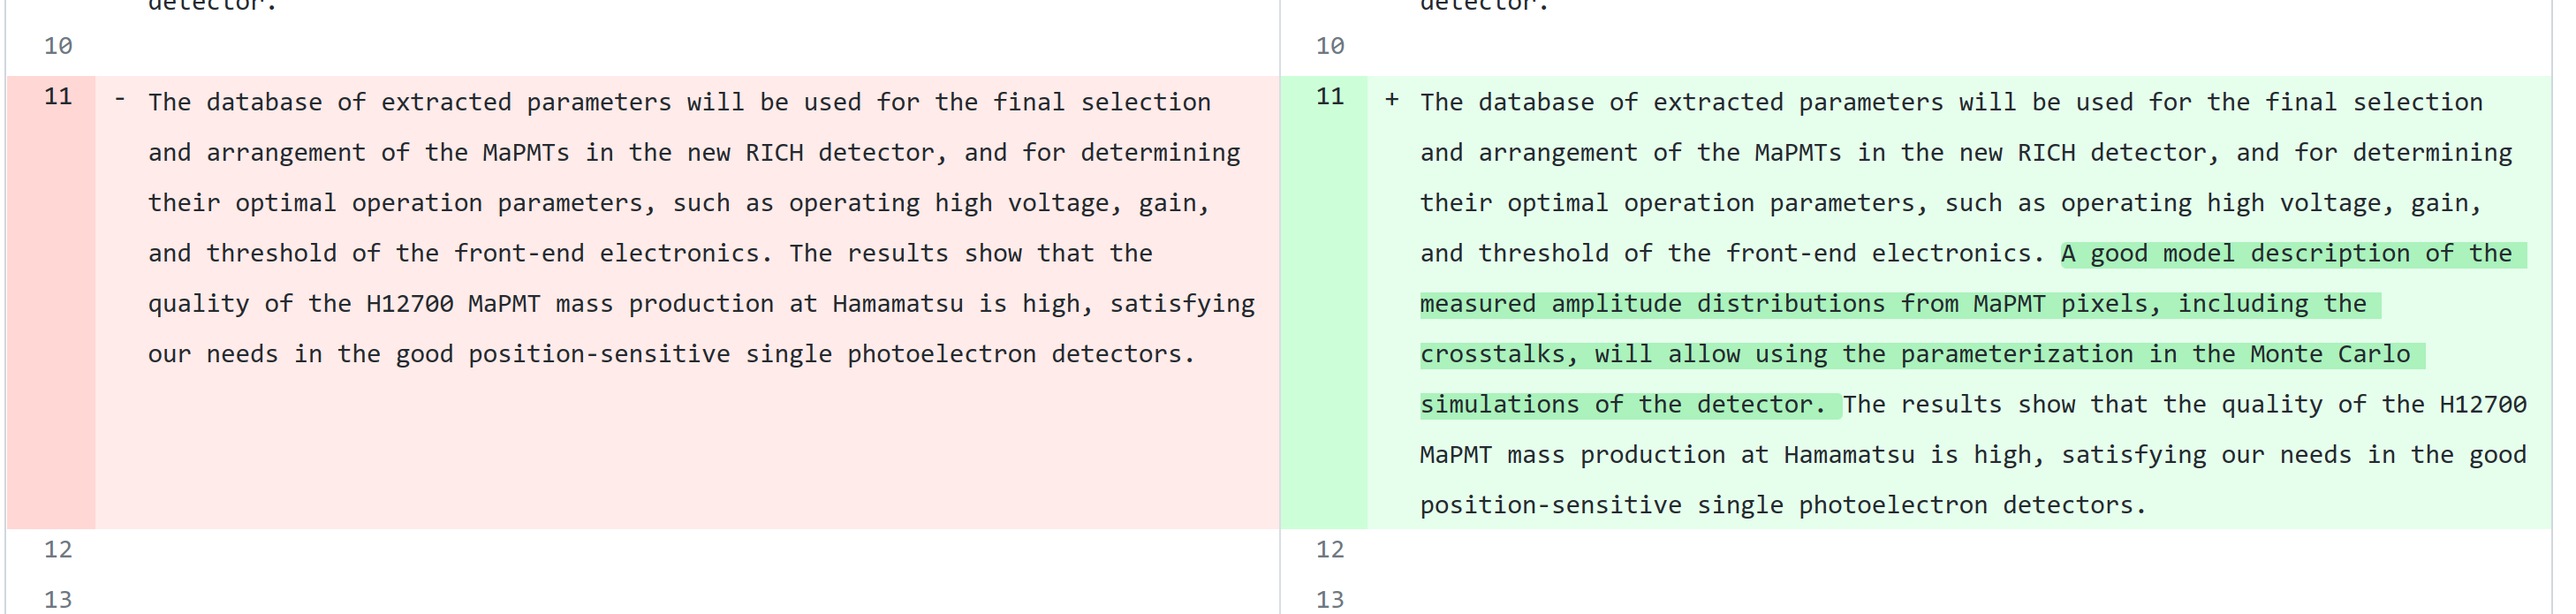
\includegraphics[width=\linewidth]{round1/1.08.png}

\begin{tcolorbox}[enlarge top by=2em,colbacktitle=black!60!white,colframe=black!80!white,left=0pt,right=0pt,top=0pt,bottom=0pt,boxrule=0.3pt,title=\bfseries1.09]
Line 447:  There are some features of the QE vs.  pixel number plot, is this understood?
\end{tcolorbox}

\fbox{\bfseries The text of the paper was changed to address the comment. See before and after version below:}

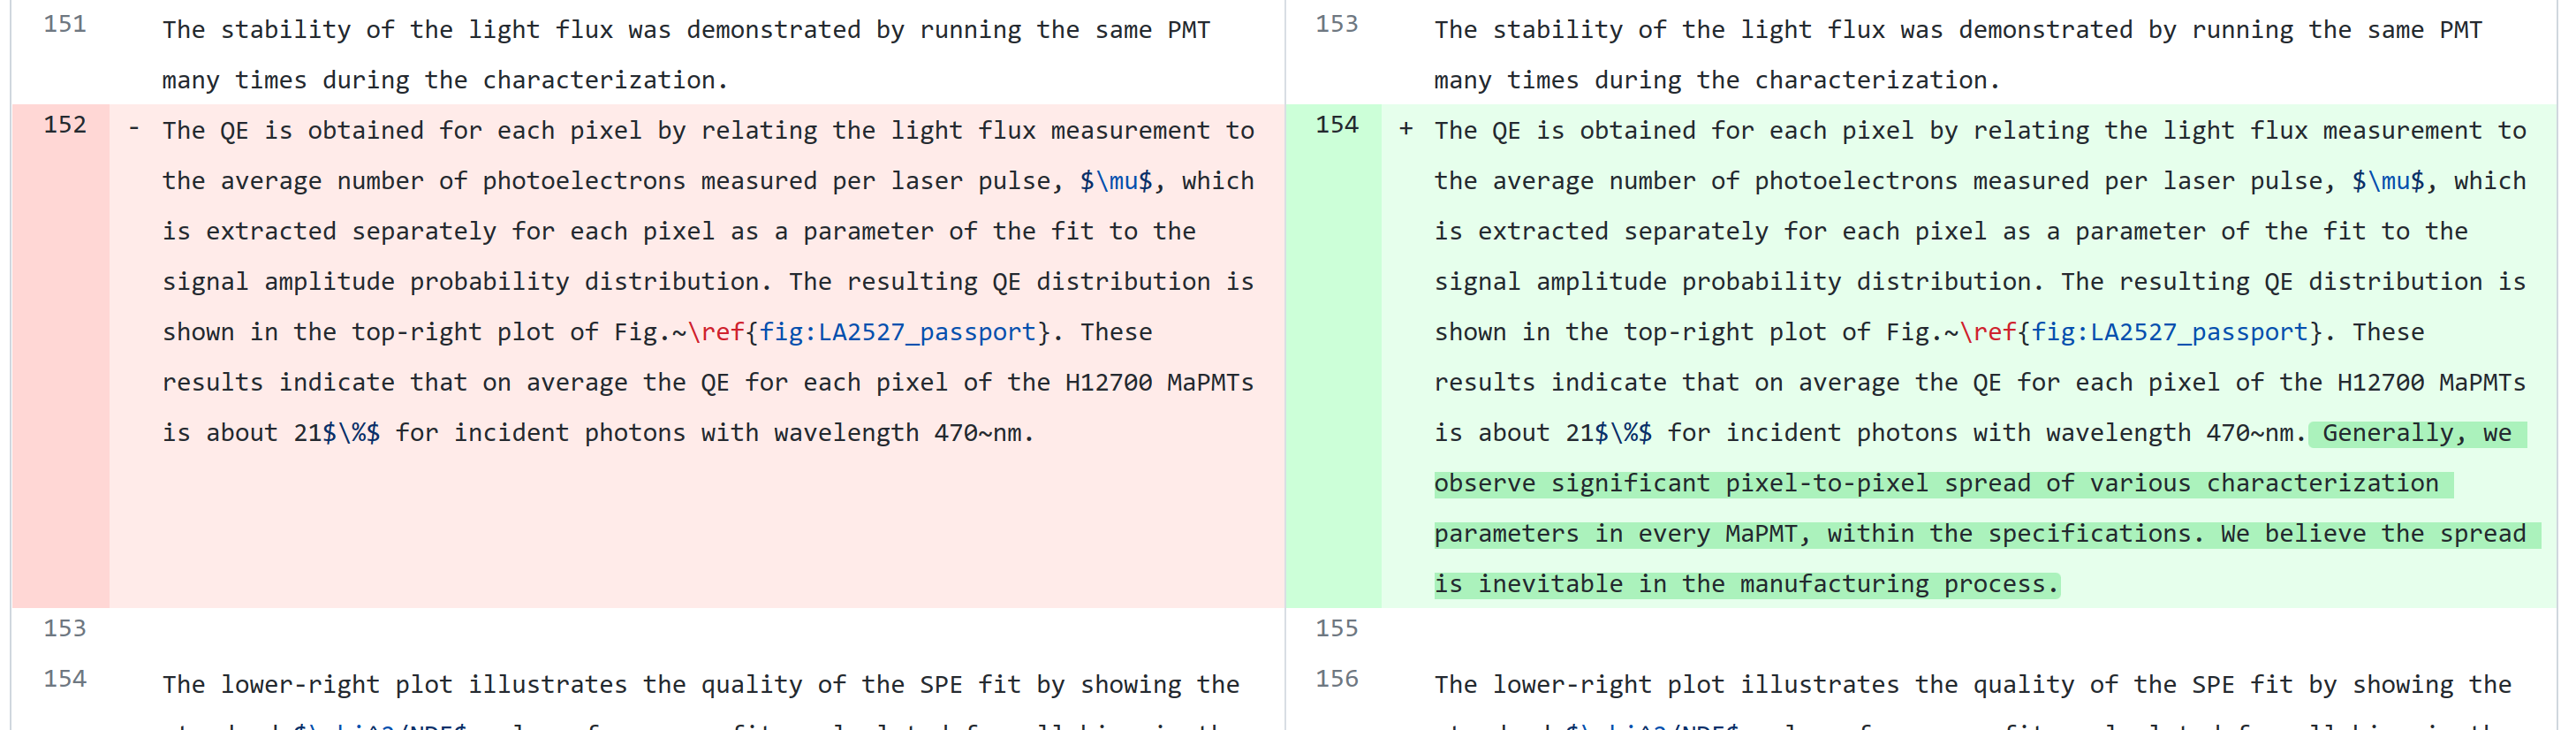
\includegraphics[width=\linewidth]{round1/1.09.png}

\begin{tcolorbox}[enlarge top by=2em,colbacktitle=blue!60!white,colframe=black!80!white,left=0pt,right=0pt,top=0pt,bottom=0pt,boxrule=0.3pt,title=\bfseries1.10]
Figure 21:  I think you can remove the word ‘Colors’ from the plot.  Same for all plot with ‘Colors’in the legend.
\end{tcolorbox}

We would prefer to keep word "Colors" for reader to know that online version is Color-coded.


\begin{tcolorbox}[enlarge top by=2em,colbacktitle=black!60!white,colframe=black!80!white,left=0pt,right=0pt,top=0pt,bottom=0pt,boxrule=0.3pt,title=\bfseries1.11]
Figure 24:  You can remove ‘essentially on top of each other’ from the caption.  I’m not certain I understand why “For the data collected at wheel position 3,  this ratio is the quantum efficiency of the individual pixels.” Is this because you’ve performed the conversion only that that wheel position? Why do you chose to do that only for wheel position 3?  Does the Q.E agree for all wheel positions?
\end{tcolorbox}

\fbox{\bfseries The text of the paper was changed to address the comment. See before and after version below:}

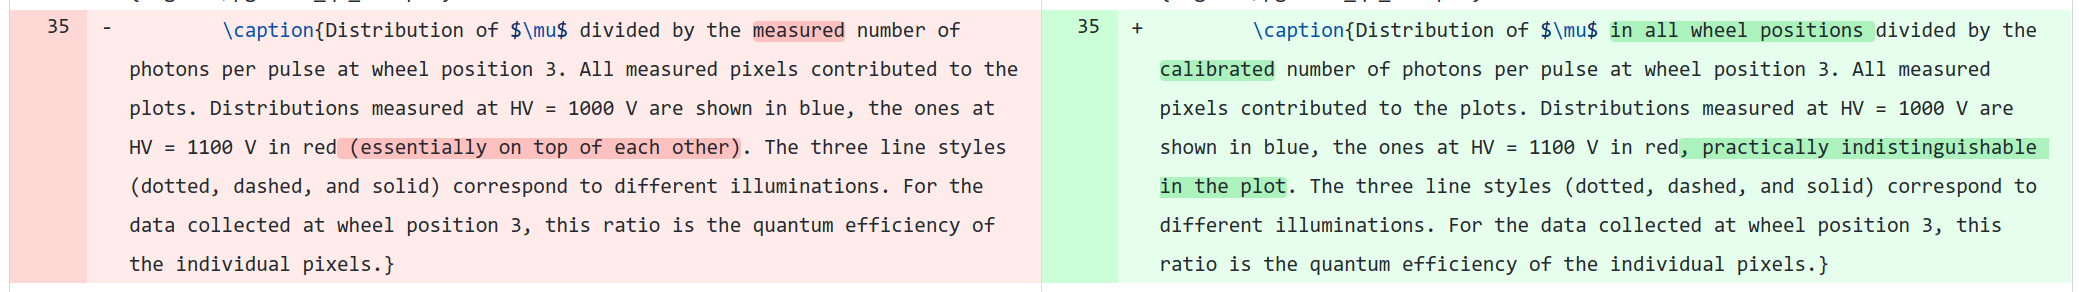
\includegraphics[width=\linewidth]{round1/1.11.png}

\begin{tcolorbox}[enlarge top by=2em,colbacktitle=black!60!white,colframe=black!80!white,left=0pt,right=0pt,top=0pt,bottom=0pt,boxrule=0.3pt,title=\bfseries1.12]
Line 550:  State clearly the value that you measure and the value that the manufacturer measurement.  Can you comment on why they might differ?
\end{tcolorbox}

\fbox{\bfseries The text of the paper was changed to address the comment. See before and after version below:}

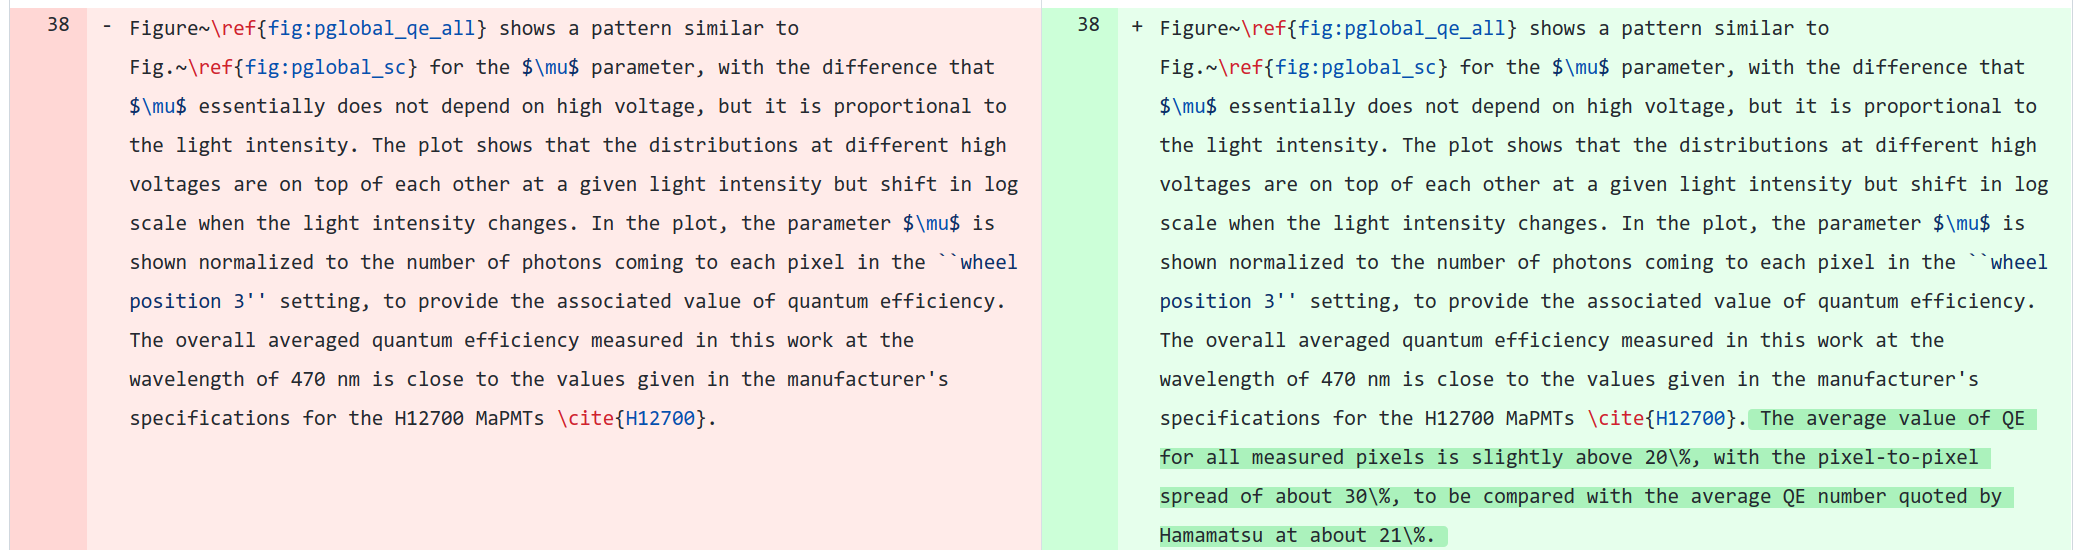
\includegraphics[width=\linewidth]{round1/1.12.png}

\begin{tcolorbox}[enlarge top by=2em,colbacktitle=black!60!white,colframe=black!80!white,left=0pt,right=0pt,top=0pt,bottom=0pt,boxrule=0.3pt,title=\bfseries1.13 and 1.14]
Line 557:  the word inefficiency does not need to be in quotes.

Line 599 and elsewhere:  I do not think quantum efficiency should be capitalized.
\end{tcolorbox}

\fbox{\bfseries The text of the paper was changed to address the comment.}







\clearpage






%%%%%%%%%%%%%%%%%%%%%%%%%%%%%%%%%%%%%
%%%%%%%%%%%%%%%%%%%%%%%%%%%%%%%%%%%%%
\begin{tcolorbox}[enlarge top by=2em,colbacktitle=blue!60!white,colframe=black!80!white,left=0pt,right=0pt,top=0pt,bottom=0pt,boxrule=0.3pt,title=\bfseries2.01]
The paper is written as a long experimental note and is characterized by a pronounced verbosity. As a general comment the paper is quite difficult to read.
\end{tcolorbox}

We believe that being the experimental note, the paper presents the state of the art work in the experimental approach to the process of selection and calibration of photomultipliers for use in the large scale Cherenkov detectors. 

Apart from that, the work introduces the new extension of the calculational model describing the PMT response to few-photoelectron events, which takes into account the description and characterization of the effect of the signal cross-talk in Multianode PMTs.
The new method of selection between the true events in a given pixel and the events when a signal is caused by the hit in a neighboring pixel will help improve the spatial resolution of single photoelectron detectors and will allow for more reliable determination of the detector signal thresholds and efficiency to the single photoelectron events.

We think we made every effort to explain and justify all our measurements and analysis to the level that can be used by other experimentalists.

In an attempt to make the paper easier to read we have added to the Introduction the brief descriptions of the upcoming Sections in the paper. Please have a look at the added paragraph at the end of this document. 


%%%%%%%%%%%%%%%%%%%%%%%%%%%%%%%%%%%%%
%%%%%%%%%%%%%%%%%%%%%%%%%%%%%%%%%%%%%
\begin{tcolorbox}[enlarge top by=2em,colbacktitle=red!60!white,colframe=black!80!white,left=0pt,right=0pt,top=0pt,bottom=0pt,boxrule=0.3pt,title=\bfseries2.02]
A list of specifications and requirements on the PMTs coming from the CLAS12 RICH are not clearly defined at the beginning of the paper, therefore the reader must guess which are the most important parameters to be measured and what characteristics will define a "good" PMT for the CLAS12 RICH production
\end{tcolorbox}

\fbox{\bfseries The text of the paper was changed to address the comment. See before and after version below:}
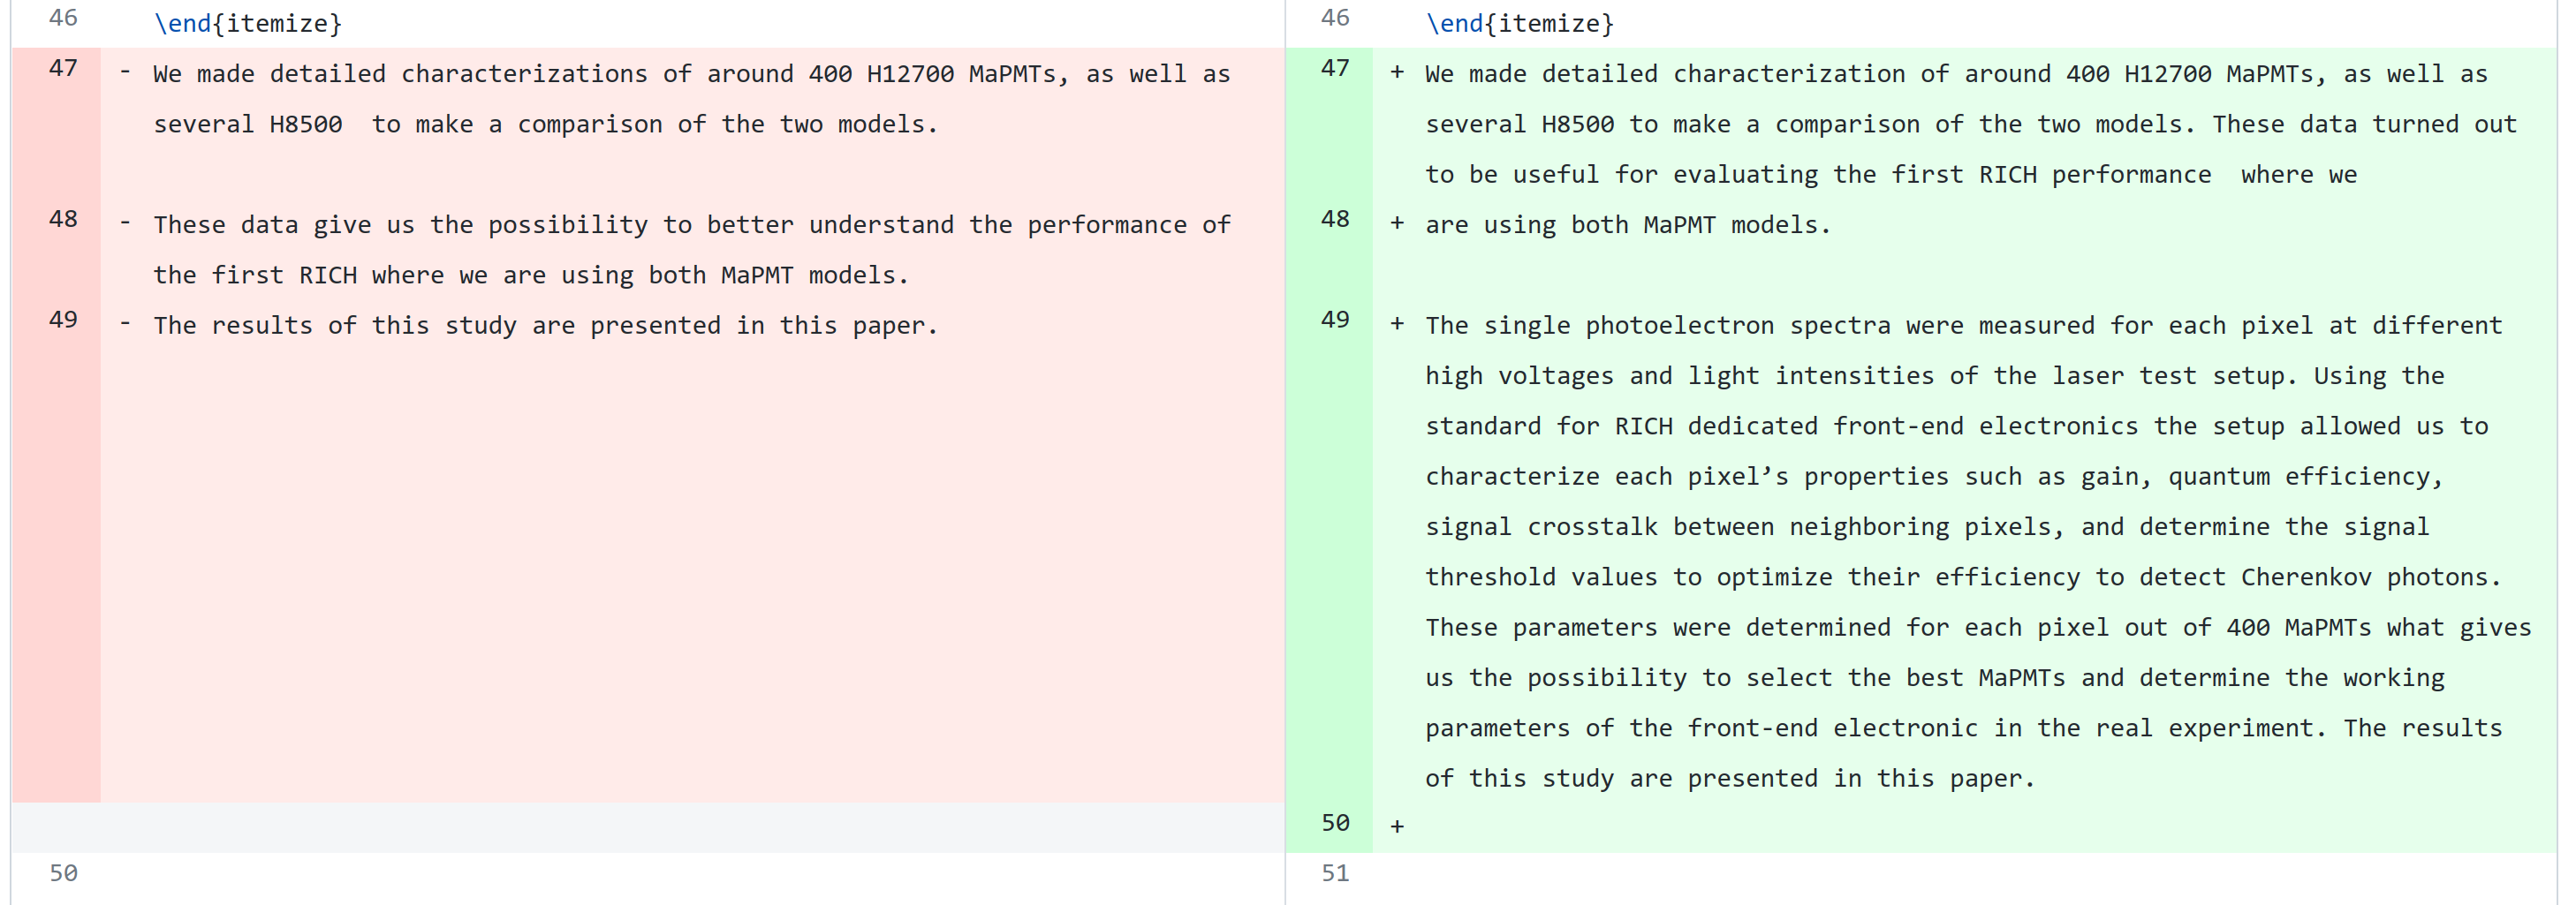
\includegraphics[width=\linewidth]{round1/2.02.png}


%%%%%%%%%%%%%%%%%%%%%%%%%%%%%%%%%%%%%
%%%%%%%%%%%%%%%%%%%%%%%%%%%%%%%%%%%%%
\begin{tcolorbox}[enlarge top by=2em,colbacktitle=red!60!white,colframe=black!80!white,left=0pt,right=0pt,top=0pt,bottom=0pt,boxrule=0.3pt,title=\bfseries2.03]
The type of MaPMTs studied in this paper (Hamamatsu H12700) have been characterized and described in the literature and are characterized by a large pixel-by-pixel and tube-by-tube gain variation (with a typical spread of 1 to 3). In addition, this type of MaPMT has some typical features of the individual pixel response which depend on the pixel position inside the matrix. Indication of the "pixel number" appears in the text and in specific plots (starting from section 4), and a channel map with channel numbers should be introduced to let the reader fully understand the measurements
\end{tcolorbox}

{\centering
\begin{tcolorbox}[enlarge top by=2em,colbacktitle=green!60!white,colframe=black!80!white,width=0.9\linewidth,left=30pt,right=30pt,top=10pt,bottom=10pt,boxrule=0.3pt,title=\bfseries our draft remarks]
I agree with the statement. The PMT channel map information might be there already, just need to highlight or give it more stress/explanation in the text.

Pixel-by-pixel and tube-by-tube gain variation and the individual pixel response 
depending on the pixel position inside the matrix is the goal of the study presented in the paper.

\end{tcolorbox}
}


%%%%%%%%%%%%%%%%%%%%%%%%%%%%%%%%%%%%%
%   2.04
%%%%%%%%%%%%%%%%%%%%%%%%%%%%%%%%%%%%%
\begin{tcolorbox}[enlarge top by=2em,colbacktitle=red!60!white,colframe=black!80!white,left=0pt,right=0pt,top=0pt,bottom=0pt,boxrule=0.3pt,title=\bfseries2.04]
This MaPMT type is also affected by after-pulses, which might have a strong impact for the CLAS12 RICH operations and not mentioned at all in the paper
\end{tcolorbox}


The after-pulse probability for MaPMT H12700 is expected to be below several percent (see for example M.~Calvi et al.,   ``Characterization of the Hamamatsu H12700A-03 and R12699-03 multi-anode photomultiplier tubes'', Journal of Instrumentation, Volume 10, Issue 09, article id. P09021 (2015)). 
During our tests we have not seen any effects of the immediate after-pulses or long-delayed after-pulses. 
No oscilloscope traces or  instabilities in the amplitude spectra showed their presence.
In general, after-pulses do not have strong impact for the CLAS12 RICH operation. They may increase the accidental noise. However, it does not affect the RICH performance due to the excellent 1~ns time resolution. Experimentally evaluated probability of accidental coincidence per one signal in a pixel, including the possible after-pulses, is very small, of the order of few times of $10^{-5}$.
%The average pixel background rate at nominal CLAS12 luminosity $10^35~cm^{-2}sec^{-1}$ is 2 kHz. It translates to 0.05 background hits in the full RICH 25,000 pixel's array. This is for the final pixel selections. At the preliminary stage we need to account the different time arrival of photons reflecting from the spherical mirrors that is around 10 ns. Even at this stage the number of background accidental hits is around 0.5. 


%{\centering
%\begin{tcolorbox}[enlarge top by=2em,colbacktitle=green!60!white,colframe=black!80!white,width=0.9\linewidth,left=30pt,right=30pt,top=10pt,bottom=10pt,boxrule=0.3pt,title=\bfseries our draft remarks]

%{\bfseries Pavel}
%Need to find a reference mentioning after-pulses and explain that such study was not considered important because the RICH signals are not in trigger and the delayed pulses do not interfere with our data. They may increase the accidental noise which is measured separately in the detector. By the way, I guess it can be observed in RICH-1 by plotting rates vs. time agter the beam stop? 

%"Characterization of the Hamamatsu H12700A-03 and R12699-03 multi-anode photomultiplier tubes"


%https://arxiv.org/pdf/1506.04302.pdf

%Although our setup (based on single photons emitted at random by a DC-biased LED) is not able to quantify the afterpulse probability for the present device, it is expected to be below 5\% for a PMT with a good quality vacuum, as explained in [7].

%{\bfseries note to editor:}

%- no immediate afterpulses (include scope picture)

%- delayed afterpulses are not important to us

%{\bfseries Pavel}
%Maybe include in the beginning somewhere: "During our tests we have not  seen any effects of the immediate after-pulses observed by other authors (see, for example, Ref.~[]). No oscilloscope traces, no instabilities in the amplitude spectra showed their presence. The long-delayed after-pulses are not critical for the RICH in which only time-synchronized events are accepted."

%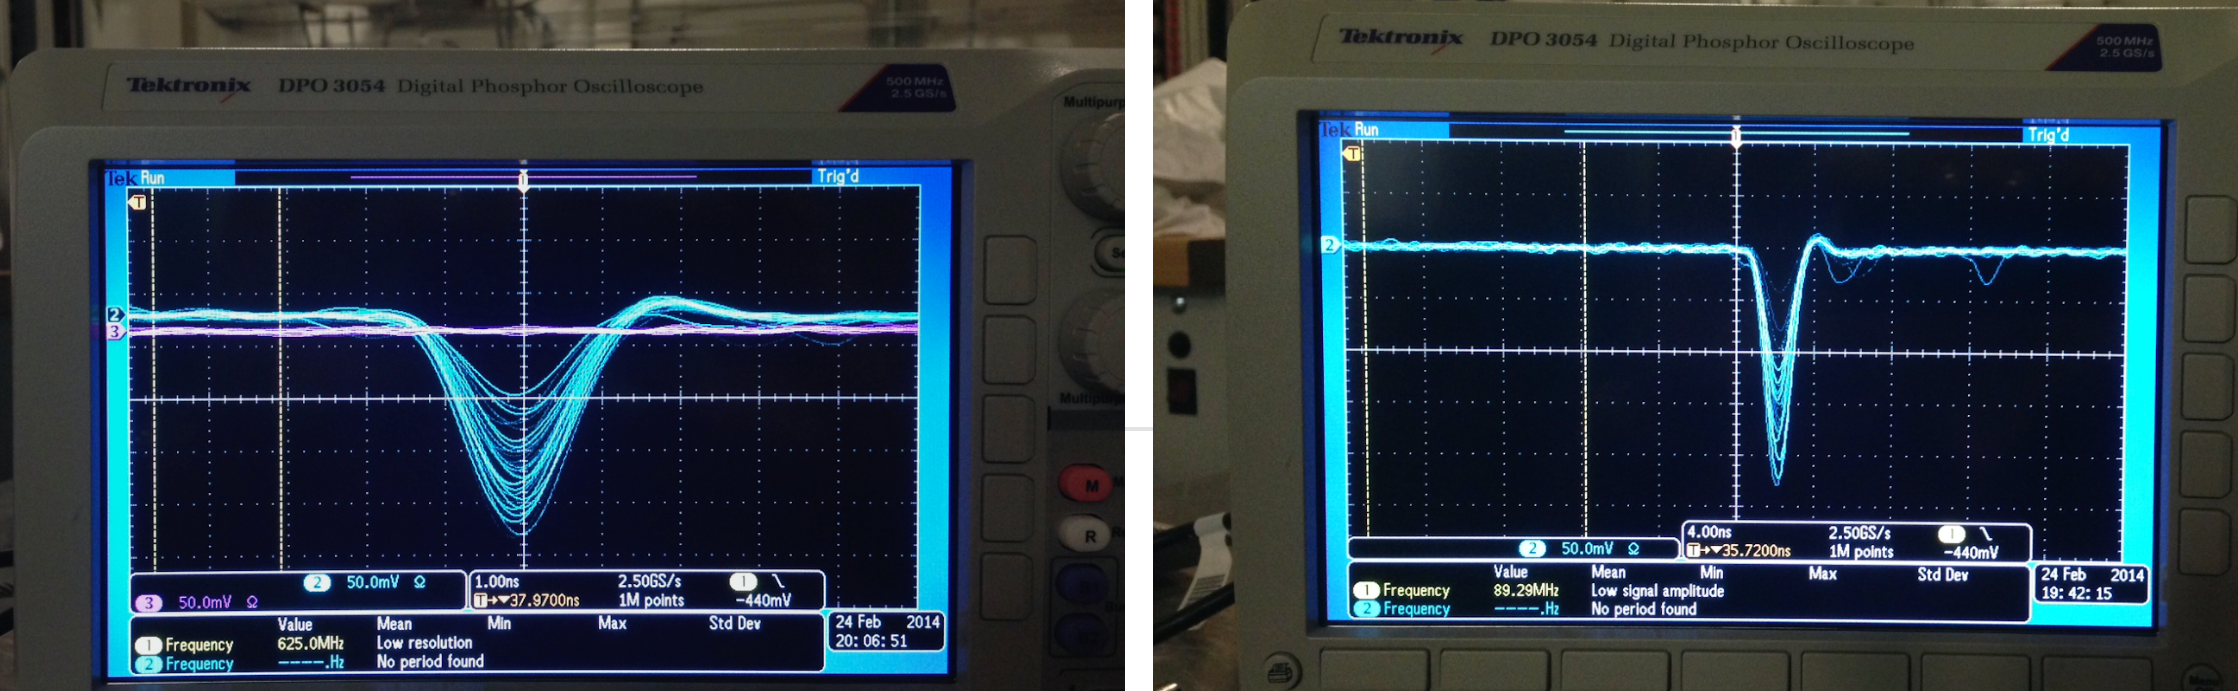
\includegraphics[width=0.7\linewidth]{round1/afterpulses.png}

%\end{tcolorbox}
%}



%%%%%%%%%%%%%%%%%%%%%%%%%%%%%%%%%%%%%
%%%%%%%%%%%%%%%%%%%%%%%%%%%%%%%%%%%%%
\begin{tcolorbox}[enlarge top by=2em,colbacktitle=blue!60!white,colframe=black!80!white,left=0pt,right=0pt,top=0pt,bottom=0pt,boxrule=0.3pt,title=\bfseries2.05]
All the main results of the paper refer to a computational model, described in detail in Ref. [12], which is adapted to the experimental conditions described in the paper (in section 6 and in the appendix). This is the part of the paper which is the most difficult to read and understand. Multiple citations of Ref. [12] are made in the text, and the reader is forced to go to that reference to fully understand in detail the procedure described in the paper.
\end{tcolorbox}

That is a correct statement.
The computational model describes the amplitude distributions of signals coming from every PMT pixel in the conditions of low light, and allows to extract its important physical parameters, such as:
\begin{itemize}
\item amplification gain in pC per one photoelectron
\item average multiplicity of the observed photoelectrons in given conditions (which can be converted to quantum efficiency)
\item shape of the single-photoelectron spectrum
\end{itemize}
All this can be consistently done in a wide range of the test conditions, using the spread of the extracted parameters to evaluate the systematical errors. The new extension of the model allows to evaluate the cross-talk effects between neighboring pixels and evaluate the optimal amplitude of separation between them.
To fully understand the outcome the familiarity with Ref. [12] is required. 



%%%%%%%%%%%%%%%%%%%%%%%%%%%%%%%%%%%%%
%%%%%%%%%%%%%%%%%%%%%%%%%%%%%%%%%%%%%
\begin{tcolorbox}[enlarge top by=2em,colbacktitle=blue!60!white,colframe=black!80!white,left=0pt,right=0pt,top=0pt,bottom=0pt,boxrule=0.3pt,title=\bfseries2.06]
Concerning plots, many of them have captions/labels too small to be easily visible by the reader
\end{tcolorbox}

The plots/captions/labels are not smaller that in the plots of Ref. 12 which is already published.
Please let us know if the sizes are not acceptable for the publisher, and we will try to fix them.


%%%%%%%%%%%%%%%%%%%%%%%%%%%%%%%%%%%%%
%%%%%%%%%%%%%%%%%%%%%%%%%%%%%%%%%%%%%
\begin{tcolorbox}[enlarge top by=2em,colbacktitle=blue!60!white,colframe=black!80!white,left=0pt,right=0pt,top=0pt,bottom=0pt,boxrule=0.3pt,title=\bfseries2.07]
The fit parameter results show some inconsistencies in Fig. 14-15-16 (especially the mu parameter in the top-right plot in each figure).
\end{tcolorbox}


Fig. 14 is not consistent with 15 and 16 because it is done with different MaPMT.
And for Fig. 15 and 16, there is actually a good consistency.
The High Voltages are different which affects the gain of the MaPMT, therefore the major change is in the $scale$ parameter, while $\mu$ (light intensity) stays the same.
The statistical spread of other parameters is expected.

The differences between the plots (a)-(d) in the Figs. 14-15-16 are discussed in the captions and in the text.
Parameter $\mu$ (light intensity) depends on the type of data (illumination settings, 3mm or 6mm mask, open pixel with software crosstalk removal, and model approximation).
In case of H8500 (Fig. 14) the model cannot extract the crosstalk correctly because it's too wide, merges with the signal, and disturbs its shape severely.



%%%%%%%%%%%%%%%%%%%%%%%%%%%%%%%%%%%%%
%%%%%%%%%%%%%%%%%%%%%%%%%%%%%%%%%%%%%
\begin{tcolorbox}[enlarge top by=2em,colbacktitle=black!60!white,colframe=black!80!white,left=0pt,right=0pt,top=0pt,bottom=0pt,boxrule=0.3pt,title=\bfseries2.08]
The chi2 of the 4 fits presented in Fig. 18 is very high, which indicates that probably the model does not represent the data well for the "highest light intensity" configuration. The illumination conditions are described in different ways that confuse the reader: a precise and unique definition should be used throughout the text
\end{tcolorbox}

 The distributions shown in Fig. 18 contain very high number of events and span several orders of magnitude in intensity. Relatively high $\chi^2/NDF$ values are not surprising in such conditions. The model is an approximation that is not expected to deliver ultimate precision in describing the spectra. Some photomultipliers may have very complicated SPE spectral shapes which cannot be represented just by three Poisson components as in our case and would need more parameters for an ideal description. The model solution for using arbitrary number of Poisson components to describe the SPE spectrum is given in Ref. 12. The three-component solution is sufficient for the description of the SPE distributions in our application case of the H12700 MaPMTs.
 

\fbox{\bfseries The text of the paper was changed to address the comment. See before and after version below:}
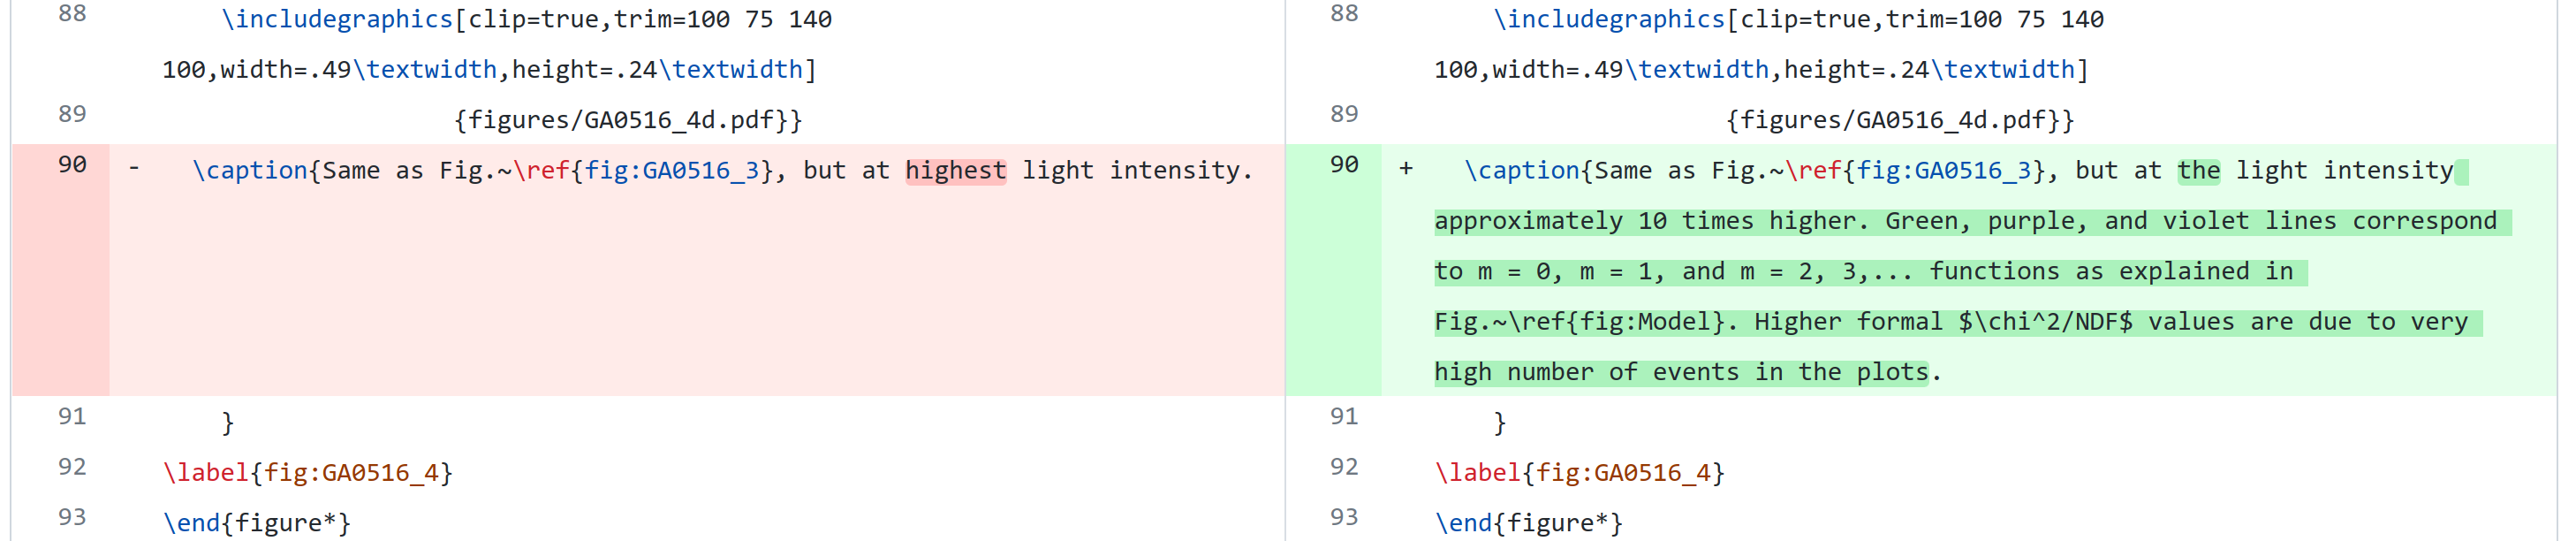
\includegraphics[width=\linewidth]{round1/2.08.png}



%%%%%%%%%%%%%%%%%%%%%%%%%%%%%%%%%%%%%
%%%%%%%%%%%%%%%%%%%%%%%%%%%%%%%%%%%%%
\newpage
\begin{tcolorbox}[enlarge top by=2em,colbacktitle=red!60!white,colframe=black!80!white,left=0pt,right=0pt,top=0pt,bottom=0pt,boxrule=0.3pt,title=\bfseries2.09]
The computational model returns a set of parameters after the fit which should be related to the ``physical observables'' typical of a PMT, like e.g. quantum efficiency (QE) or gain. Most of the ``measurements'' presented in the paper are the result of a fit using the above-mentioned model, and are not compared with independent measurements, which would be necessary to assess the correctness of the model. Only self-consistency checks of the model are partially shown in the paper. 
\end{tcolorbox}




The computational model describing the distributions of charge collected during the experiments in the low light conditions uses the set of parameters which includes the physical observables characterizing the PMT (or a pixel in the PMT) objectively. As it has been demonstrated in Ref. 12, and also shown in this work, the model allows to extract the gain (``scale'') from different independent experiments using widely varying illuminations. Changing average number of photons in a test pulse results in the very different charge distributions. However, the computational analysis and the fitting procedure produce the values of gain essentially identical (spread by less than 1\% if measured in the same location in the test matrix, and less than 2\% if measured in all six locations). 


Varying the high voltage also produces different charge distributions, the gain goes up by about a factor 2 upon the HV increase by 100 V. But the values of the extracted average number of photoelectrons ($\mu$ parameter) from these independent experiments are also identical within similar systematical errors. 

Other parameters exhibit similar objective characteristics, such as the gain on the first dynode $\nu$, the parameters characterizing the crosstalk, and the shapes of the SPE spectra as shown in Fig. 20: the shapes are extracted independent of the illumination, but they change with the value of HV.

That is the reason we believe we can declare our parameters to be the physical observables. Their values are obtained in the set of independent experiments, and the systematical errors are evaluated from the statistical spread of the results. The comparison of the six independent measurements for every pixel also tests the ability of the model to predict: once the set of parameters is obtained for one setup, the distributions can be predicted and then verified for a setup with the light intensity, say, twice as large, and so on. The discussion of the variability of the results and the systematical errors is given in Section 8.

The crude cross-verification of the model was performed by the satisfactory comparisons of the expositions at the extra low illumination with the simplest model assuming that all the events in the charge spectra above the threshold belong to the SPE distribution and calculating average $scale$ and $\mu$ which were consistent with the model results. The method was not used in the mass production as it required longer times, and resulted in lower redundancy and reliability. In addition, that simple method does not allow to check the consistency of the extracted spectra, especially in the case of MaPMTs sometimes exhibiting very complex SPE shapes.    

\fbox{\bfseries The text of the paper was changed to address the comment. See before and after version below:}
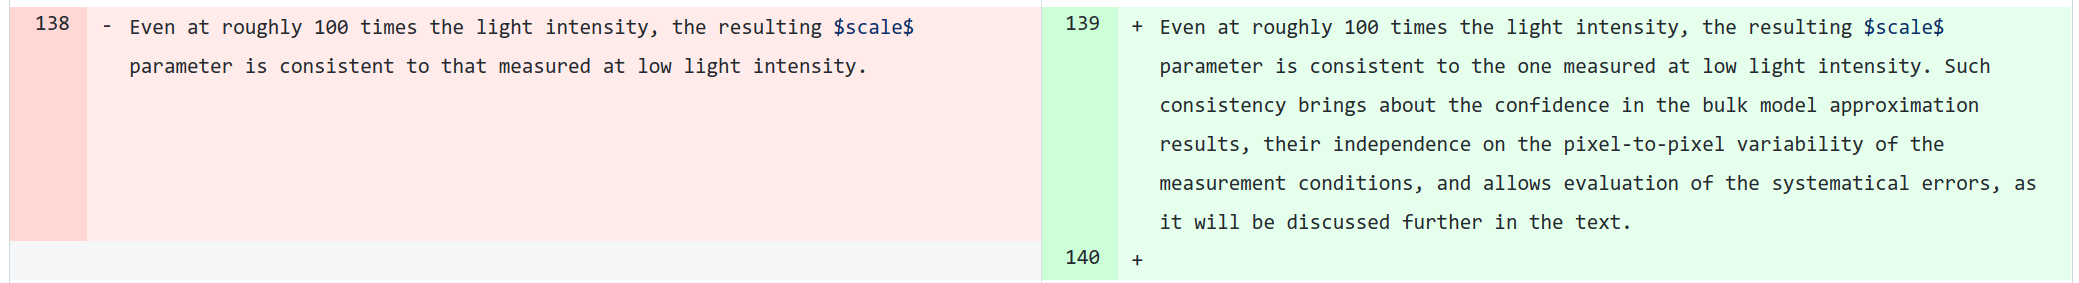
\includegraphics[width=\linewidth]{round1/2.09.png}



%%%%%%%%%%%%%%%%%%%%%%%%%%%%%%%%%%%%%
%%%%%%%%%%%%%%%%%%%%%%%%%%%%%%%%%%%%%
\begin{tcolorbox}[enlarge top by=2em,colbacktitle=black!60!white,colframe=black!80!white,left=0pt,right=0pt,top=0pt,bottom=0pt,boxrule=0.3pt,title=\bfseries2.09a]
Just to quote a few examples: The top-right plot in Fig. 19 shows QE measurements as a function of the anode number for a PMT. No error bars (except probably the ones on the fit parameters) are indicated to understand the precision in the estimate of this important quantity (no evaluation of systematic errors). A comparison with an independent measurement would be important, even on a limited number of MaPMTs (e.g. measurement of the absolute QE made using a calibrated monocromatic light source)
\end{tcolorbox}

\fbox{\bfseries The text of the paper was changed to address the comment. See before and after version below:}
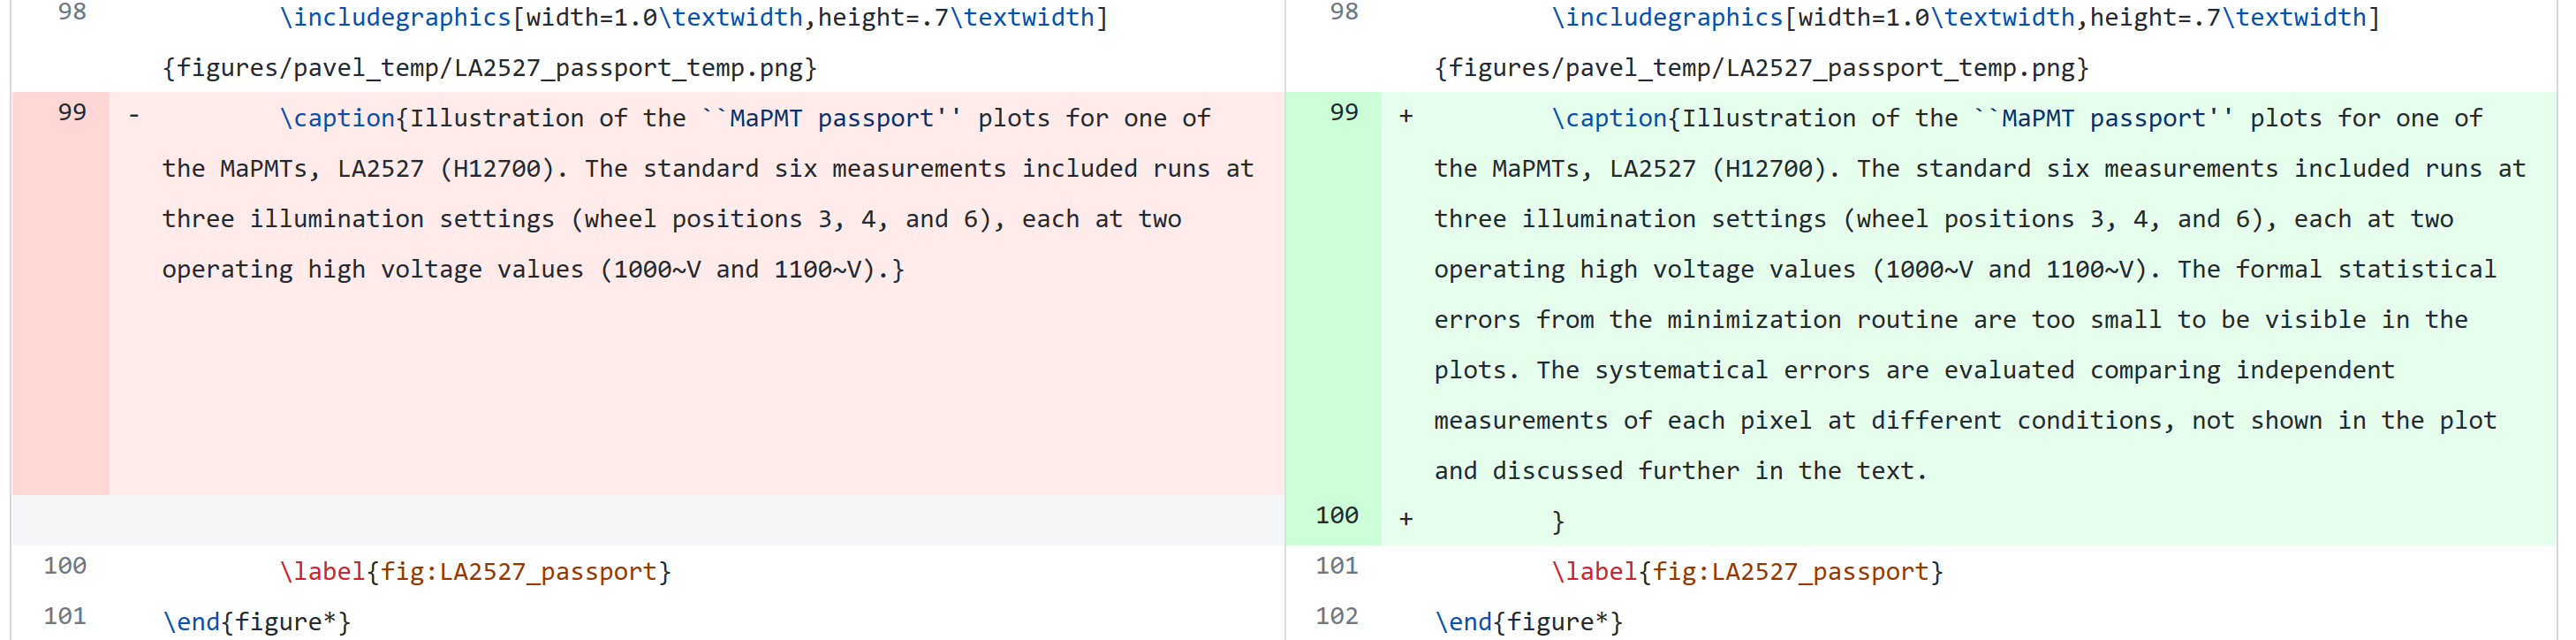
\includegraphics[width=\linewidth]{round1/2.09a.png}



%%%%%%%%%%%%%%%%%%%%%%%%%%%%%%%%%%%%%
%%%%%%%%%%%%%%%%%%%%%%%%%%%%%%%%%%%%%
\begin{tcolorbox}[enlarge top by=2em,colbacktitle=black!60!white,colframe=black!80!white,left=0pt,right=0pt,top=0pt,bottom=0pt,boxrule=0.3pt,title=\bfseries2.09b]
The top-left plot in Fig. 19 shows the scale (proportional to the PMT anode gain) as a function of the anode number for a PMT. Some variation is shown, still without error bars (or with error bars only coming from the fit parameters, with no systematic error evaluation). However, a larger pixel-to-pixel variation is expected for this type of PMT
\end{tcolorbox}

\fbox{\bfseries The text of the paper was changed to address the comment. See before and after version below:}

\fbox{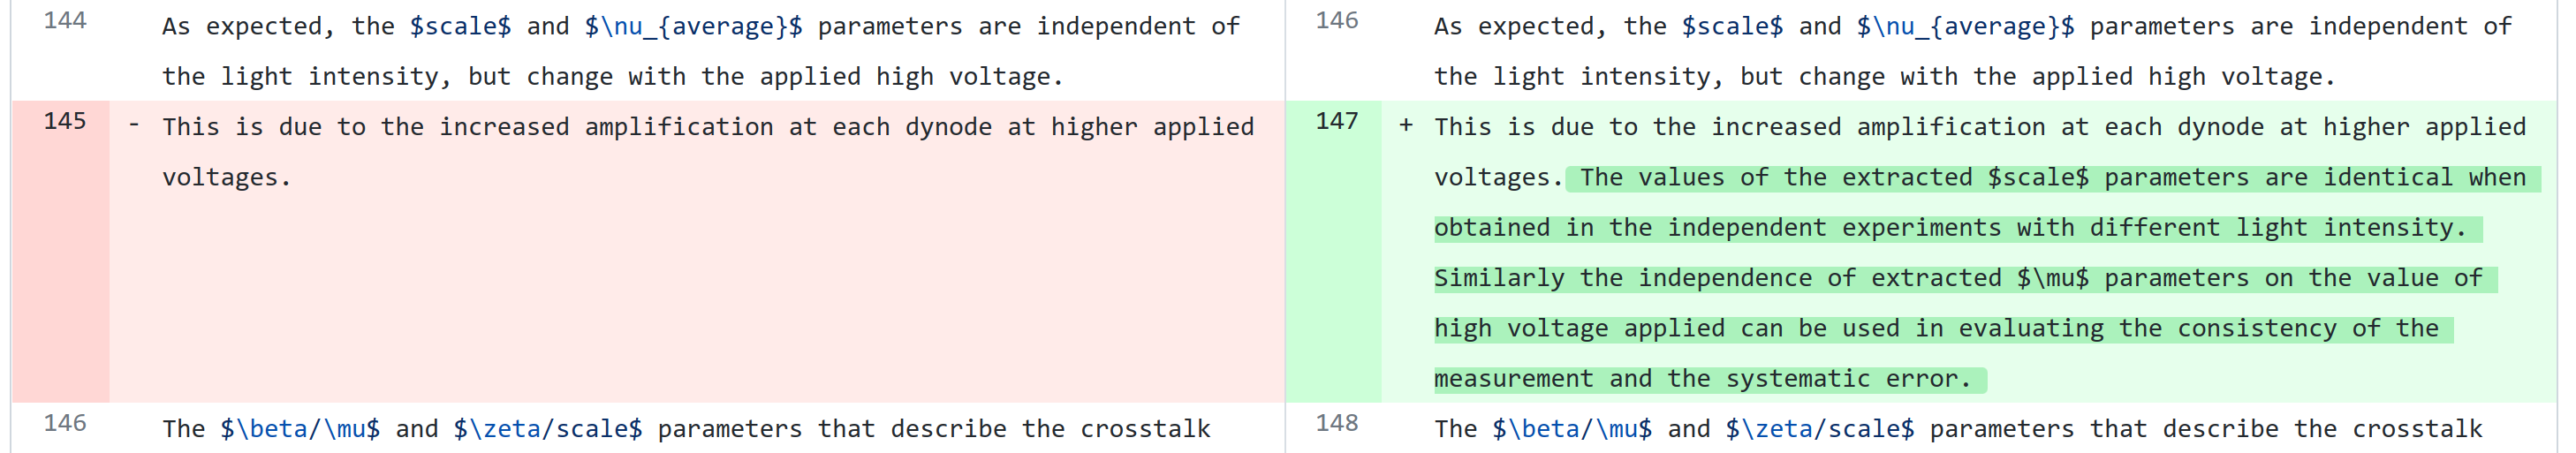
\includegraphics[width=\linewidth]{round1/2.09b.png}}

\fbox{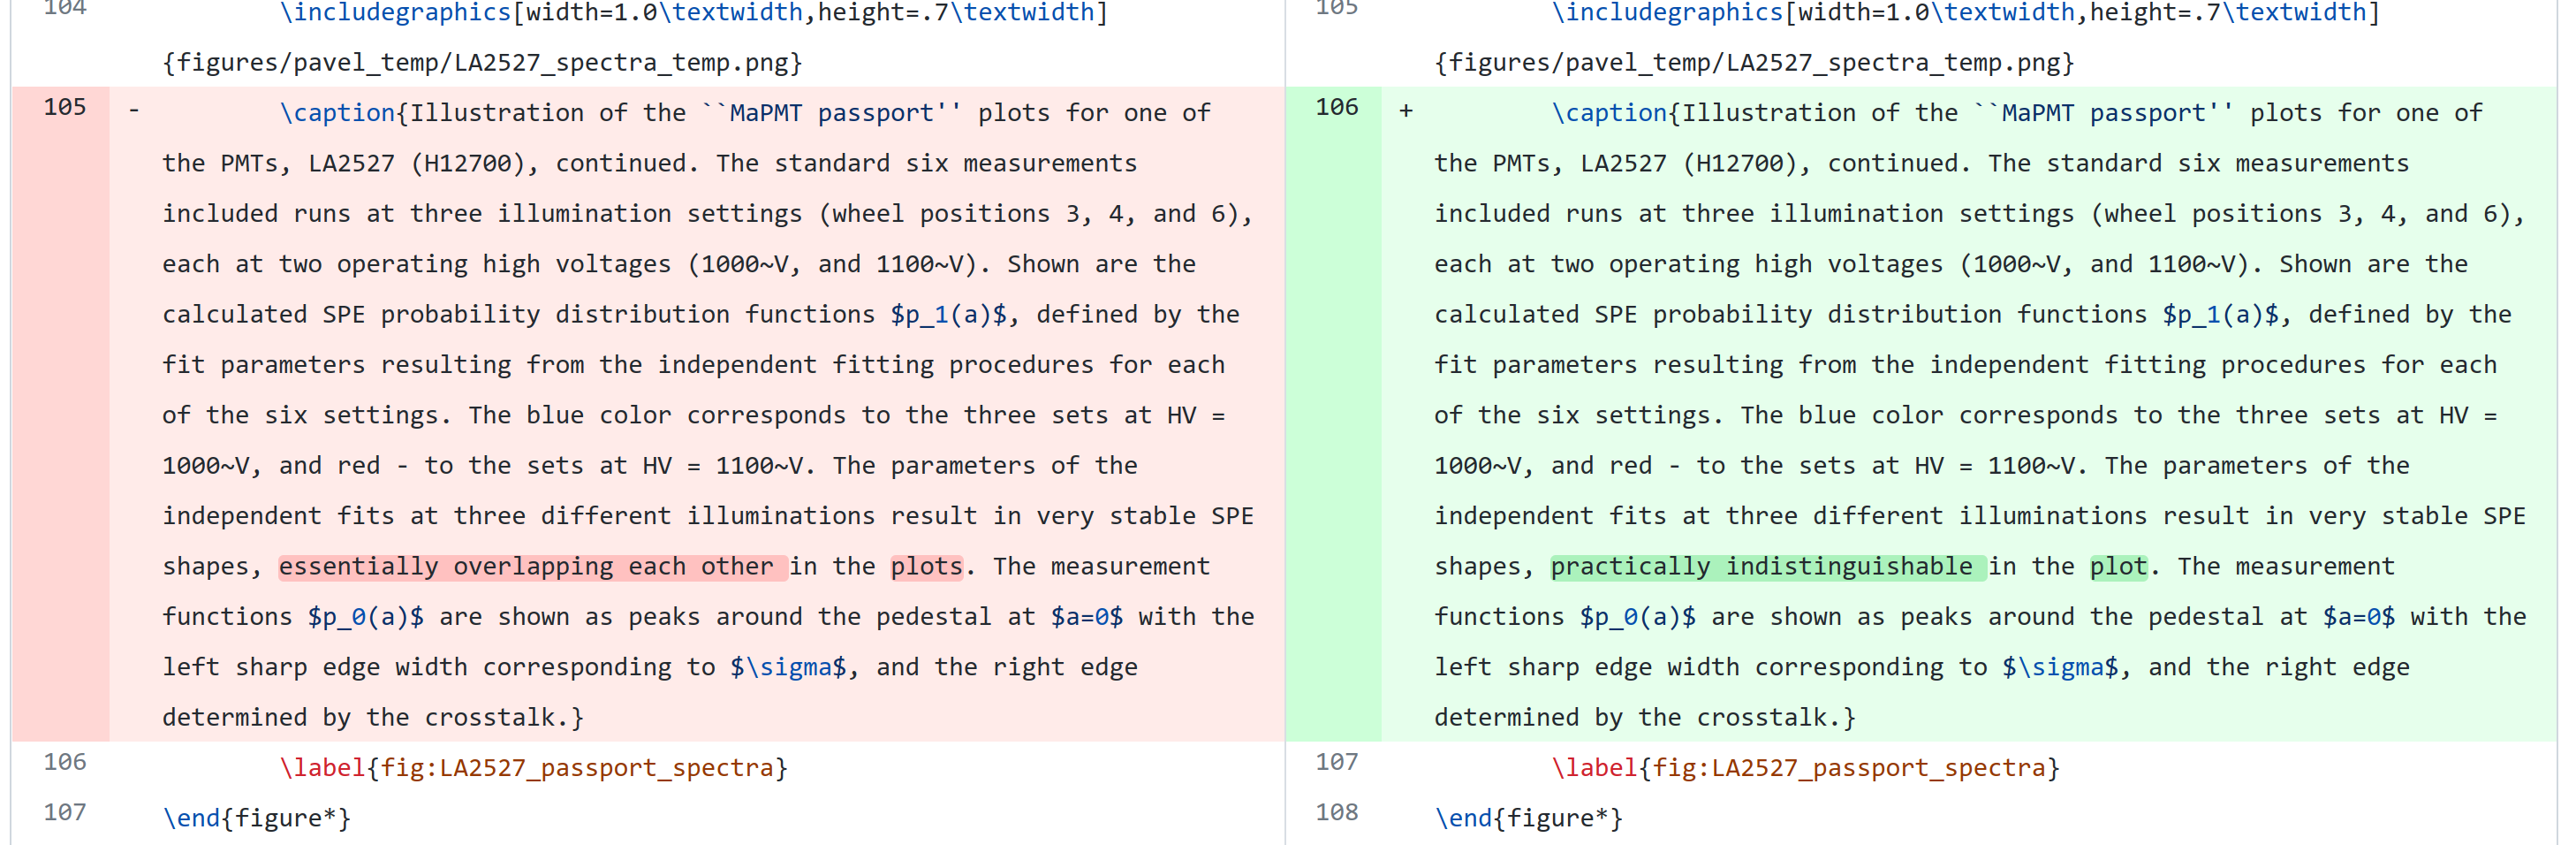
\includegraphics[width=\linewidth]{round1/2.09c.png}}



%%%%%%%%%%%%%%%%%%%%%%%%%%%%%%%%%%%%%
%%%%%%%%%%%%%%%%%%%%%%%%%%%%%%%%%%%%%
\begin{tcolorbox}[enlarge top by=2em,colbacktitle=blue!60!white,colframe=black!80!white,left=0pt,right=0pt,top=0pt,bottom=0pt,boxrule=0.3pt,title=\bfseries2.10]
In conclusion, the paper presents measurements on a large PMT population (about 400 detectors), which are essentially based on a computational model described in another paper (Ref. [12]).
\end{tcolorbox}

{\bfseries Please see our response to 2.01.}


%%%%%%%%%%%%%%%%%%%%%%%%%%%%%%%%%%%%%
%%%%%%%%%%%%%%%%%%%%%%%%%%%%%%%%%%%%%
\begin{tcolorbox}[enlarge top by=2em,colbacktitle=blue!60!white,colframe=black!80!white,left=0pt,right=0pt,top=0pt,bottom=0pt,boxrule=0.3pt,title=\bfseries2.11]
In its current form the paper does not satisfy the Journal requirements and should not be published. A major revision is needed, strongly reducing the written text to improve conciseness and reducing the number of plots, inserting only representative ones. What is missing in particular is the list of specifications on the PMTs coming from the physics of the experiment, and the requirements that the PMTs must satisfy to pass the "selection" to be mounted inside the second RICH of CLAS12, as the reader might expect reading the title.
\end{tcolorbox}

We respectfully disagree with the request to strongly reduce the written text and number of plots.
We believe such change would make the work less comprehensible.
The list of the PMT specifications and requirements has been added to the introduction as stated in the reply to 2.02.

%%%%%%%%%%%%%%%%%%%%%%%%%%%%%%%%%%%%%
%%%%%%%%%%%%%%%%%%%%%%%%%%%%%%%%%%%%%
\begin{tcolorbox}[enlarge top by=2em,colbacktitle=blue!60!white,colframe=black!80!white,left=0pt,right=0pt,top=0pt,bottom=0pt,boxrule=0.3pt,title=\bfseries2.12]
In addition, the validation of the model using independent data on individual parameters is needed to assess the precision of the used method (just to quote an example, a comparison of QE with independently measured values, e.g. by Hamamatsu or by a calibrated monocromatic light source), which lacks evaluation of systematic uncertainties on the presented parameters.
\end{tcolorbox}


The comparison of the QE with Hamamatsu data is given in the paper during the discussion od Fig. 19 in Section 7.
Unfortunately the precise comparison of the anode gains with Hamamatsu data is not possible since they are using different techniques and report values convoluted with quantum efficiencies with unknown scale of light intensities. But qualitatively the agreement is good.

The systematical uncertainties for each measured parameter are evaluated by the comparison of its values obtained in six independent measurements performed for each MaPMT. Two HV by three illumination settings produced three independent values for the 



\clearpage




%%%%%%%%%%%%%%%%%%%%%%%%%%%%%%%%%%%%%
%%%%%%%%%%%%%%%%%%%%%%%%%%%%%%%%%%%%%
\begin{tcolorbox}[enlarge top by=2em,colbacktitle=red!60!white,colframe=black!80!white,left=0pt,right=0pt,top=0pt,bottom=0pt,boxrule=0.3pt,title=\bfseries Addition 1]
\end{tcolorbox}

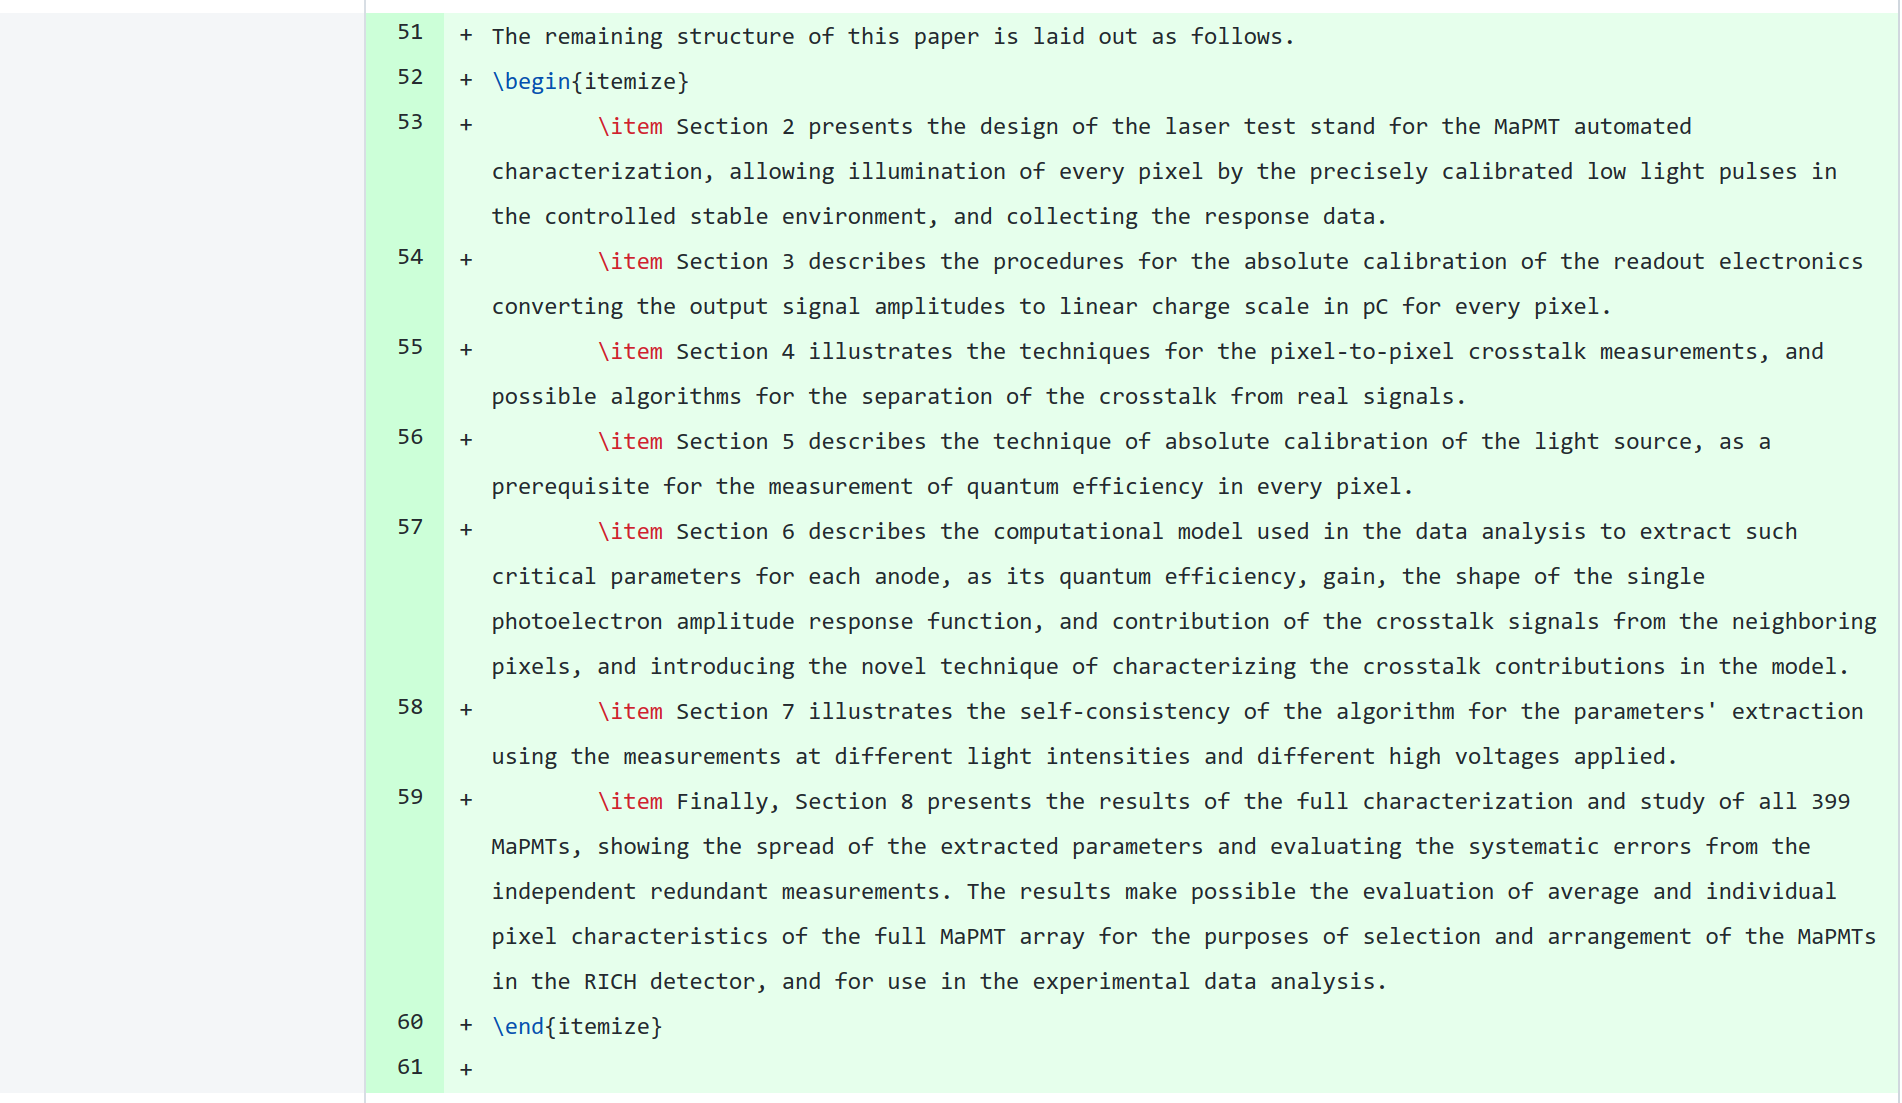
\includegraphics[width=\linewidth]{round1/add1.png}

\end{document} 
